\documentclass{article}
\usepackage{qilin}
\tikzstyle{process} = [rectangle, rounded corners, minimum width=1.5cm, minimum height=0.5cm,align=center, draw=black, fill=gray!30, auto]
\title{MAT347: Groups, Rings and Fields}
\author{QiLin Xue}
\date{Fall 2021}
\usepackage{mathrsfs}
\usetikzlibrary{arrows}
\usepackage{stmaryrd}
\usepackage{accents}
\newcommand{\ubar}[1]{\underaccent{\bar}{#1}}
\usepackage{pgfplots}
\numberwithin{equation}{section}

\begin{document}

\maketitle
\tableofcontents
\newpage
\section{Group Theory}
Group theory and symmetry are closely related. Consider the following equilateral triangle made up of some stiff material, allowing it to perform rigid motion.
\begin{center}
    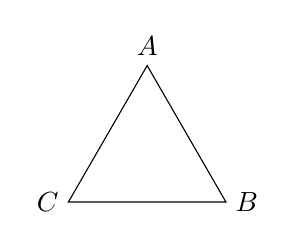
\begin{tikzpicture}
        \draw[-] (0,0) node[left]{$C$}-- (2,0)node[right]{$B$} -- (1,1.732) node[above]{$A$} -- cycle;
    \end{tikzpicture}
\end{center}
There are six symmetries:
\begin{itemize}
    \item rotations $2\pi/3: A\to C\to B\to A$
    \item rotations $4\pi/3: A\to B\to C\to A$
    \item reflections $C\leftrightarrow B, C\leftrightarrow A,$ or $A\leftrightarrow B$
    \item identity transformation: $A\to A, B\to B, C\to C:$ denoted as either $\id$ or $e.$
\end{itemize}
Let $\rho$ be a rotation through $2\pi/3$ and $\sigma$ a reflection $C \leftrightarrow B.$ We want to compose them as $\rho \sigma,$ which takes $ABC\to ACB \to CBA.$ Therefore, $A \leftrightarrow C,$ so this becomes another reflection. Similarly, $\sigma\rho$ takes $ABC \to CAB \to BAC,$ which results in an overall $A\leftrightarrow B,$ resulting in another but \textit{different} reflection.

Here, $\sigma$ and $\rho$ are symmetries. Applying these to a triangle will still give us a triangle, so it makes sense that their composition will be a symmetry as well. However, the order of composition may make a difference. Some terminology: if $\sigma\rho = \rho\sigma,$ we say the two elements \emf{commute}.

For a square, there are eight symmetries:
\begin{center}
    \begin{tikzpicture}
        \draw[] (0,0) node[below]{$D$} -- (2,0)node[below]{$C$} -- (2,2)node[above]{$B$} -- (0,2)node[above]{$A$} -- cycle;
    \end{tikzpicture}
\end{center}
Namely, the identity $e$, 3 rotations, and 4 reflections. Note that in each symmetry, $\alpha$ has an inverse $\alpha^{-1}$ with the property that $\alpha\alpha^{-1}=e=\alpha^{-1}\alpha.$
\begin{definition}
    A \emf{group} is a set $G$ with a composition:
    \begin{align*}
        G\times G & \to G                     \\
        (g,h)     & \mapsto gh \sim g \circ h
    \end{align*}
    satisfying:
    \begin{enumerate}
        \item Associativity: $(gh)k = g(hk)$
        \item Identity: $\exists e \in G$ such that $eg=ge=g, \forall g \in G$
        \item For every $g\in G, \exists g^{-1}\in G$ such that $g^{-1}g=gg^{-1}=e$
    \end{enumerate}
\end{definition}
We can look at some examples.
\begin{itemize}
    \item $\mathbb{Z}$ with $+$ is a group, where $e=0$ and $n^{-1}=-n.$ Likewise, this is true for any field.
    \item The multiplicative group $F^\times= F\setminus \{0\}$ has identity $1$ and the inverse of $x$ is $x^{-1}=1/x.$
    \item $\mathbb{Z}/n\mathbb{Z}$ (addition modulo $n$)
    \item $SL(n,F)$ (special linear group) = all $n\times n$ matrices over a field $F$ whose determinant equals $1.$
    \item $GL(n,F)$ (general linear group) = all invertible $n\times n$ matrices
    \item $SO(n,F)$ (special orthogonal group) = $\{A\in SL(n,F) | A^T = A^{-1}\}$
\end{itemize}
\begin{example}
    $\mathbb{Z}/n\mathbb{Z} = \{0,1,\dots,n-1\}$ is one of the simplest groups where addition is done under modulo $n$. That is, if $n=8$ we have $5+7=12 \equiv 4.$

    \textit{Notation:} we can write elements with a bar at the top. For example, $\bar{5}+\bar{7} = \bar{4}.$ Note that $\bar{k}^{-1} = \overline{-k} = \overline{n-k}.$
    \vspace{2mm}

    An alternative way to express elements is through the bijection:
    \begin{equation*}
        \bar{k} \leftrightarrow e^{2\pi i k/n},
    \end{equation*}
    and the group operation is multiplication in $\mathbb{C}^\times.$ Here, $\mathbb{Z}/n\mathbb{Z}$ is known as a cyclic group.
\end{example}
We often denote the \emf{cyclic group} of order $n$ by $C_n.$ The \emf{order} of a group $G$ is its cardinality, denoted as $|G|$ or $\text{ord}(G).$ Using this notation,
\begin{align*}
    |C_n| &= n \\ 
    |\text{triangle group}| &= 6 \\
    |\text{rigid motions of square}| &= 8 \\ 
    |(\mathbb{R},+)| &= \infty. 
\end{align*}
\begin{example}
    The \emf{quaternion group} is written as
    \begin{equation}
        \mathbb{H} = \{\pm 1, \pm i, \pm j, \pm k\},\quad\quad |\mathbb{H}|=8,
    \end{equation}
    with $1=\text{id},$ and the group operation is given by
    \begin{align*}
        ij &= -ji = k \\ 
        jk &= -kj = i \\ 
        ki &= -ik = j \\ 
        i^2 &= j^2 = k^2 = -1.
    \end{align*}
    Note that $\mathbb{H}$ sometimes refers to
    \begin{equation*}
        \{a1 + bi + cj + dk | a,b,c,d\in \mathbb{R}\},
    \end{equation*}
    which is closely related but not the same. We will be working with the first definition.
\end{example}
Recall that in our triangle group, we can find a smaller group (cyclic of order 3) $\{e,\rho,\rho^2\}$ that also forms a group. This is known as a \emf{subgroup.}
\begin{definition}
    A nonempty subset $H$ of a group $G$ is a subgroup and we write $H \le G,$ if H is a group using the same operations as G. This means that if $h,k\in H,$ then $hk \in H$ and $h^{-1} \in H.$
\end{definition}
\begin{proposition}
    If $\emptyset \neq H \subseteq G,$ then $H \le G$ if and only if $hk^{-1} \in H, \forall h,k \in H.$
\end{proposition}
As a non-example, if $F$ is a field, then $F^\times = F\setminus \{0\}$ is a non-empty subset of $F$ and is also a group, but it is not a subgroup of $F^+,$ since the group operation is different.
\begin{example}
    Recall that in $\mathbb{H},$ we have $i,i^2=-1,i^3=-i,i^4=1,$ so $\{1,i,-1,-i\}$ is a cyclic subgroup of order $4.$ Sometimes, we write this as $\langle i\rangle,$ which is the group \emf{generated} by $i$.
\end{example}
A direct corollary is that if $g_1,\dots,g_m \in G,$ then $\langle g_1,\dots,g_m\rangle$ is the smallest subgroup of $G$ that contains $g_1,\dots,g_m.$ Here, $g_1,\dots,g_m$ are known as the \emf{generators} of the subgroup, but are not uniquely determined.

\begin{definition}
    Let $G$ be a group and $H\le G.$ Consider sets of the form
    \begin{equation*}
        Hg = \{hg|h\in H\}
    \end{equation*}
    for some fixed $g\in G.$ This is a \emf{coset} of H. And in particular, it is a \emf{right coset}.
\end{definition}
Let us investigate properties of cosets. Consider $Hg$ and $Hg'$ for some $g,g'\in G.$ These cosets might be disjoint, but we will first look at the case in which they intersect. In other words, $hg=h'g'$ for some $h,h'\in H$. Multiplying both sides by $h^{-1}$, we have
\begin{align*}
    g=h^{-1}h'g' \in Hg',
\end{align*}
since $h^{-1}h'\in H.$ Similarly, we have $g'\in Hg.$

Now consider an arbitrary element of $Hg,$ which we write as $kg,$ with $k\in H.$ Then:
\begin{align*}
    kg = kh^{-1}h'g' \in Hg'.
\end{align*}
This is true for all $k\in Hg,$ so $Hg \subseteq Hg'.$ By symmetry, we also have $Hg' \subseteq Hg,$ so $Hg=Hg'.$ This leads us to an important result,
\begin{proposition}
    The (right) cosets of $H$ partition $G,$ so 
    \begin{equation*}
        G = \bigsqcup Hg,
    \end{equation*}
    where $\{g_i\}$ are representative elements of disjoint cosets.
\end{proposition}
Recall that for a fixed $g$, if $hg=h'g,$ then $h=h'.$ This means in $Hg,$ each $h\in H$ gives a different element $hg,$ so 
\begin{equation*}
    |Hg| = |H|.
\end{equation*}
Therefore, \begin{equation*}
    |G| = (\text{\# of distinct right cosets}) \cdot |H|.
\end{equation*}
This proves Lagrange's Theorem,
\begin{theorem}
    If $|G|<\infty$ and $H \le G,$ then $|H|$ divides $|G|.$
\end{theorem}
We write 
\begin{equation*}
    \frac{|G|}{|H|} = [G:H],
\end{equation*}
which is the \emf{index} of $H$ in $G.$ Therefore, 
\begin{equation*}
    |G| = [G:H] |H|.
\end{equation*}
This also works for infinite groups, if $G$ and $H$ are infinite. We can use this to quickly classify subgroups. For example, if $|G|=13,$ the only subgroups of $G$ are $|e|$ and $G.$
\begin{example}
    Let $G=\mathbb{Z}$ and $H=2\mathbb{Z}$ is the group of even integers, then the distinct cosets are:
    \begin{itemize}
        \item $H+0=H$ are the even integers
        \item $H+1$ are the odd integers, so 
    \end{itemize}
    \begin{equation*}
        \mathbb{Z} = 2\mathbb{Z} \bigsqcup (2\mathbb{Z}+1),
    \end{equation*}
    so $[\mathbb{Z}:2\mathbb{Z}]=2.$
\end{example}
Note that everything above is also true for left cosets. How then, do left and right cosets interact?

To motivate this, we look at the triangle group and consider the subgroup $H=\{e,\sigma_A\}$. Then the distinct right cosets are:
\begin{itemize}
    \item $He=H = \{e, \sigma_A\}$
    \item $H\rho = \{\rho, \sigma_B\}$
    \item $H\rho^2 = \{\rho^2, \sigma_C\}$ 
\end{itemize}
Similarly, the distinct left cosets are:
\begin{itemize}
    \item $eH = H = \{e, \sigma_A\}$
    \item $\rho H = \{\rho, \sigma_C\}$
    \item $\rho^2 H = \{\rho^2, \sigma_B\}$
\end{itemize}
In general, $gH \neq Hg.$
\begin{definition}
    An \emf{action} of a group $G$ on a set $X$ is a map
    \begin{align*}
        G \times X \rightarrow X \\ 
        (g,x) &\mapsto g\cdot x = gx,
    \end{align*}
    subject to 
    \begin{enumerate}[label=(\roman*)]
        \item $(gh)\cdot x = g(h\cdot x)$
        \item $e \cdot x = x$
    \end{enumerate}
\end{definition}
If $G$ is a group, then it acts on itself. Specifically, 
\begin{equation*}
    (g,x) \mapsto g \cdot x = gx,
\end{equation*}
where we used the group product. This is known as the \emf{left translation} or the \emf{left regular action.}

We can also define the \emf{right regular action} As
\begin{equation*}
    (g,x) = xg^{-1}.
\end{equation*}
Finally, we can define how $G$ acts on $G$ by 
\begin{equation*}
    (g,x) = gxg^{-1},
\end{equation*}
and is reminiscent of the change of basis formula in multivariable calculus. This action is called \emf{conjugation.}
\begin{example}
    Let $G = SO(3),$ and $X=S^2.$ We have that $G$ acts on $X$ by rotation. Let 
    \begin{equation*}
        H = \begin{pmatrix}
            \cos\theta & \sin\theta & 0 \\ 
            -\sin\theta & \cos\theta & 0 \\
            0 & 0 & 1,
        \end{pmatrix},
    \end{equation*}
    which are rotations about the $z$ axis and also acts on $X.$
\end{example}
\begin{definition}
    If $G$ acts on $X$ and $x\in X,$ then the \emf{orbit} of $x$ under $G$ is the set of all points $x$ is taken to by elements of $G$, written as:
    \begin{equation*}
        G \cdot x = \{g\cdot x \mid g\in G\}.
    \end{equation*}
\end{definition}
Therefore, the orbits of $SO(2)$ on the sphere are the lines of latitudes and the poles $N$ and $S.$ Similarly, the orbit of $SO(3)$ is the whole sphere.

Consider the orbit of $N$. Recall that $H$ fixes $N$. Recall that the leftcoset is 
\begin{equation*}
    gH = \{gh|h\in H\}.
\end{equation*}
Since $h$ fixes $N$, $ghN=gN.$ Every element of $gH$ takes $N$ to the same point $gN.$ Suppose that $gH$ and $g'H$ are cosets such that $gHN = g'HN,$ which implies $gN=g'N,$ or $(g')^{-1}gN=N.$ We can say that $g'^{-1}g=h.$ Therefore, the points on the sphere are in a 1-1 correspondence with the left cosets of $H$.
\begin{definition}
    If $G$ acts on $X$ and $x\in X$ then the \emf{stabilizer} of $x$ in $G$ is 
    \begin{equation*}
        \text{Stab}_G(x) = \{g\in G| gx=x\}
    \end{equation*}
\end{definition}
\section*{Cayley's Theorem}
If we have $G$ acting on $X,$ then there is an isomorphism 
\begin{equation*}
    \varphi: G \to S_X \cong S_n,
\end{equation*}
where $n=|X|.$ For example, let $H \le G$ and $X=G/H$ where $G$ acts by left translation. This is transitive, and 
\begin{equation*}
    \ker \varphi = \bigcap_{x} xHx^{-1}.
\end{equation*}
For the specific case where $H=\{e\}.$ Therefore, 
\begin{equation*}
    \ker\varphi = \{e\}
\end{equation*}
and $\varphi$ us 1-1 and 
\begin{align*}
    \varphi: G \to S_X
\end{align*}
is an isomorphism, from $G$ to $\Im f,$ a subgroup of $S_X.$
\begin{theorem}
    Every group is isomorphic to a subgroup of $S_n$ for some $n.$
\end{theorem}
Consider another example, where $G$ acts on itself by conjugation,
\begin{align*}
    g \cdot x = gxg^{-1} = C_g(x).
\end{align*}
This is no longer transitive (or else everything is conjugate to everything else). The orbits are the conjugacy classes and are disjoint, since conjugacy is an equivalence relation. Note that if $z\in Z(G),$ then 
\begin{equation*}
    gzg^{-1} = z
\end{equation*}
for all $g.$ Therefore, $\{z\}$ is a conjugacy class with one element if and only if $z\in Z(G).$ If $G$ is abelian, then $Z(G)=G$ and every element is its own conjugacy class.

Because conjugacy is an equivalence relation,
\begin{equation*}
    G = \bigsqcup (\text{conjugacy classes}).
\end{equation*}
If $\{e=z_1,\dots,z_k\} = Z(g)$ and $g_1,g_2,\dots,g_m$ are representatives of the non-central conjugacy classes, we can write 
\begin{equation*}
    C(g_i) = \{gg_ig^{-1}|g\in G\}.
\end{equation*}
Then,
\begin{equation*}
    G =\left(\bigsqcup \{z_i\}\right) \sqcup \left(\bigsqcup C(g_i)\right),
\end{equation*}
which if you have gone past kindergarten math, you can count
\begin{equation*}
    |G| = |Z(G)| + \sum_i |C(g_i)|.
\end{equation*}
This leads to the \emf{class equation}. We first need to state the \emf{orbit-stabilizer} theorem,
\begin{theorem}
    For all $x\in X,$ the map 
    \begin{align*}
        G/\text{Stab}(x) &\to G \cdot x \\ 
        g\text{Stab}(x) &\mapsto g\cdot x,
    \end{align*}
    is a well-defined bijection. Thus,
    \begin{equation*}
        |G\cdot x| = [G:\text{Stab}(x)]
    \end{equation*}
    and if $|G|<\infty,$ then 
    \begin{equation*}
        |G\cdot x| = |G|/|\text{Stab}(x)|
    \end{equation*}
\end{theorem}
\begin{theorem}
    The better \emf{class equation} is 
    \begin{equation*}
        |G| = |Z| + \sum_{i=1}^n [G:Z(g_i)]
    \end{equation*}
\end{theorem}
We can apply this to $S_3.$ The center is $Z(S_3)=\{e\}.$ The index of a 2-cycle is $3$ and the index of a 3-cycle is $2.$ Therefore,
\begin{equation*}
    |S_3| = 1 + 2 + 3 = 6.
\end{equation*}
We introduce $p$ groups,
\begin{definition}
    A finite group $G$ is a $p$-group if $|G|=p^n$ for some $n\in \mathbb{Z}_{\ge 0}.$
\end{definition}
There is an interesting theorem,
\begin{theorem}
    If $G$ is a non-trivial $p$-group, then $Z(G)$ is non-trivial.
\end{theorem}
\begin{proof}
    Note that 
    \begin{equation*}
        |Z| = |G| - \sum [G:Z(g_i)],
    \end{equation*}
    but both terms are powers of $p,$ so 
    \begin{equation*}
        |Z| \equiv 0 \pmod{p}.
    \end{equation*}
\end{proof}
\end{document}